% decrease in accuracy
Figure \ref{fig:nclasses} shows the graph of accuracy versus number of classes.  Each of those points is a model trained with the indicated number of classes. The classes used to train each model were take at random. The bottom line indicates, for comparison, what the accuracy would be for a random guessing classifier. The points for 2 classes use transparency to improve visualisation, as many of them are too close.

It is important to notice that, for most cases, the five models plotted for each column is a very small subset of all possible combinations for that number of classes. 

\todo{include results of previous studies in graph}


\noindent
\begin{figure*}[htb!]
\centering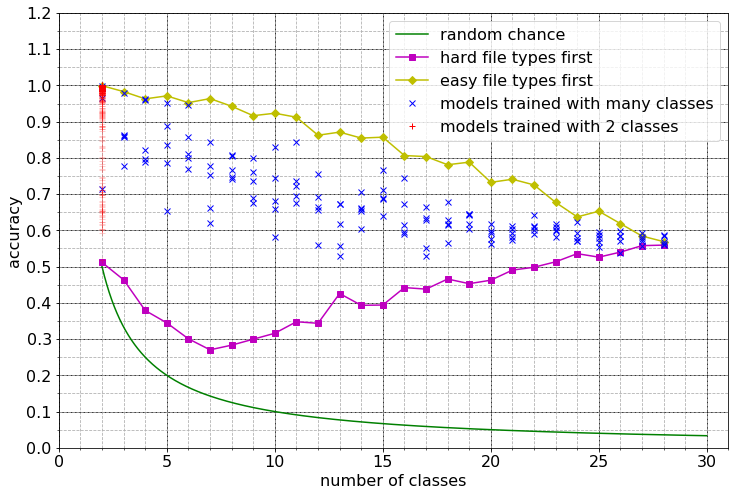
\includegraphics[width=1.0\textwidth]{content/nclasses.png}
\caption{\label{fig:nclasses}Validation accuracy by number of classes}%
\end{figure*}

Figure \ref{fig:dual} shows the graph of the accuracy of each class when compared individually with each one of the others, the 378 possible pairs of classes. File types where all the poins are close to 1.0 are hardly mistaken for other types, while file types presenting some accuracies close to 0.5 can be mistaken for other file types in the perspective of the used model.

\noindent
\begin{figure*}[htb!]
\centering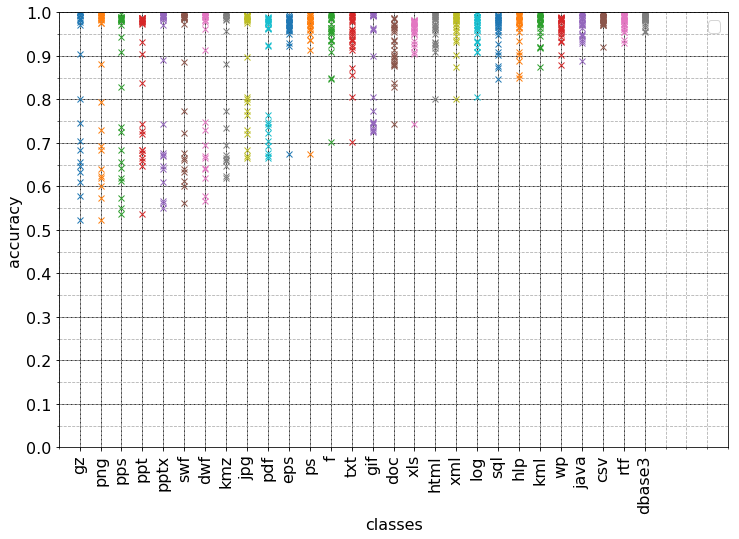
\includegraphics[width=1.0\textwidth]{content/dual.png}
\caption{\label{fig:dual}Validation accuracy of models trained with pair of classes}%
\end{figure*}



A 28x28 matrix was made using the accuracy of the models built for each pair of classes as a distance measure. Then a PCA dimensionality reduction technique was used to plot this data in a 2D graph, grouping similar file types.
The result is shown in figures \ref{fig:pca} and \ref{fig:pca2}. 

\noindent
\begin{figure*}[htb!]
\centering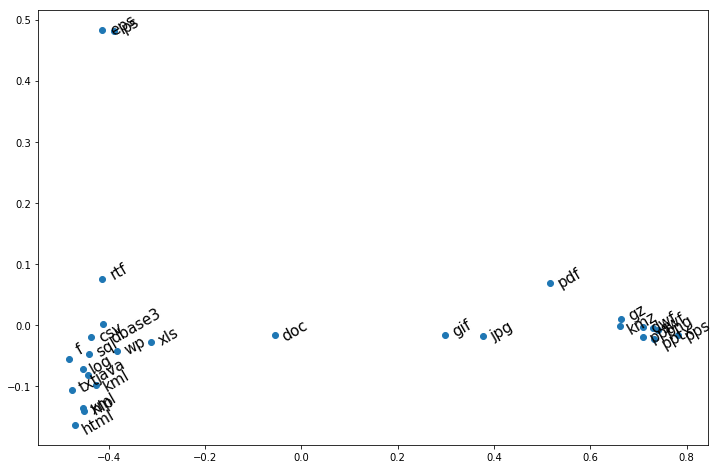
\includegraphics[width=1.0\textwidth]{content/pca.png}
\caption{\label{fig:pca}PCA of accuracy of models trained with pair of classes}%
\end{figure*}


\noindent
\begin{figure*}[htb!]
\centering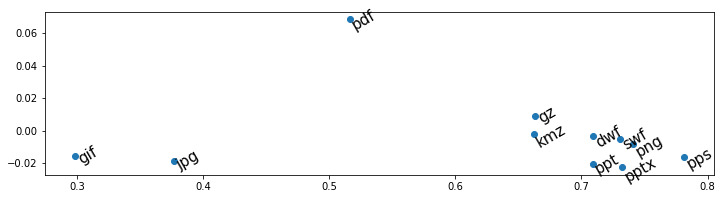
\includegraphics[width=1.0\textwidth]{content/pca2.png}
\caption{\label{fig:pca2}PCA of accuracy of models trained with pair of classes - detail}%
\end{figure*}


% the problem of unseen file types
% \levelC{Limitations and threats to validity}
